% Folded figure (Fig.2): G1G2 top edge, base BC, dashed levels through A and E.
% Right-angle mark at A between G1A (dashed) and BG2 (solid), as in original.
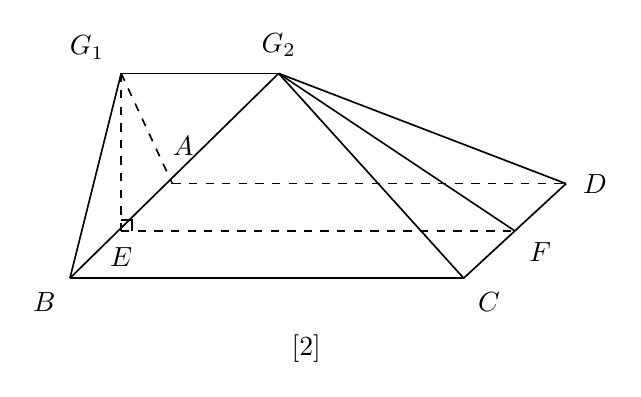
\begin{tikzpicture}[x=1cm,y=1cm,font=\normalsize,
  solidedge/.style={solid,line width=.6pt},
  hidedge/.style={dashed,line width=.6pt},
  ptlabel/.style={font=\normalsize,inner sep=2pt}]
\coordinate (B) at (0,0);
\coordinate (C) at (5,0);
\coordinate (E) at (0.6500000000,0.6000000000);
\coordinate (Flow) at (6.0,0.32);
\coordinate (F) at (5.6500000000,0.6000000000);
\coordinate (A) at (1.3000000000,1.2000000000);
\coordinate (D) at (6.3000000000,1.2000000000);
\coordinate (Dup) at (1.3,1.0);
\coordinate (Gone) at (0.6500000000,2.6000000000);
\coordinate (Gtwo) at (2.6500000000,2.6000000000);
% dashed levels
\draw[hidedge] (E)--(F);
\draw[hidedge] (A)--(D);
% foot of perpendicular and lower construction
\draw[hidedge] (Gone)--(A);
\draw[hidedge] (Gone)--(E);
% visible edges
\draw[solidedge] (B)--(C);
\draw[solidedge] (B)--(Gone);
\draw[solidedge] (Gone)--(Gtwo);
\draw[solidedge] (B)--(Gtwo);
\draw[solidedge] (Gtwo)--(C);
\draw[solidedge] (Gtwo)--(F);
\draw[solidedge] (F)--(C) (F)--(D);
\draw[solidedge] (Gtwo)--(D);
% right-angle mark at A
\draw[solidedge] ([shift={(0,.14)}]E)--++(.14,0)--++(0,-.14);
% labels kept off the strokes
\node[ptlabel,above left] at ([xshift=-4pt,yshift=3pt]Gone) {$G_{1}$};
\node[ptlabel,above] at ([yshift=4pt]Gtwo) {$G_{2}$};
\node[ptlabel,below left] at ([xshift=-3pt,yshift=-3pt]B) {$B$};
\node[ptlabel,below right] at ([xshift=3pt,yshift=-3pt]C) {$C$};
\node[ptlabel,right] at ([xshift=4pt]D) {$D$};
\node[ptlabel,below,xshift=0pt,yshift=0pt] at ([yshift=-4pt]E) {$E$};
\node[ptlabel,below right] at ([xshift=3pt,yshift=-2pt]F) {$F$};
\node[ptlabel,above right,xshift=-5pt,yshift=7pt] at ([xshift=3pt,yshift=1pt]A) {$A$};
\node[ptlabel,font=\normalsize] at (3,-0.9) {\bitmapinsertcaption[2]};
\end{tikzpicture}
